\documentclass[professionalfont,table,svgnames,xcolor=svgnames,aspectratio=169]{beamer}
%\pdfpageattr {/Group << /S /Transparency /I true /CS /DeviceRGB>>}
\usepackage{multimedia}
\usepackage{hyperref}
%%% Поля и разметка страницы %%%
\usepackage{lscape}		% Для включения альбомных страниц
\usepackage{geometry}	% Для последующего задания полей
%\usepackage[a4paper, mag=1000,left=2.5cm, right=1cm, top=2cm, bottom=2cm, headsep=0.7cm, footskip=1cm ]{geometry}

%%% Кодировки и шрифты %%%
\usepackage{metalogo}
\usepackage{cmap}						% Улучшенный поиск русских слов в полученном pdf-файле
%\usepackage[T2A]{fontenc}				% Поддержка русских букв
%\usepackage[utf8]{inputenc}				% Кодировка utf8
\usepackage{textcomp}
\usepackage[english, russian]{babel}	% Языки: русский, английский
%\usepackage[14pt]{extsizes}

\usepackage{xltxtra}
\usepackage{xunicode}
\usepackage{color}
\usepackage{colortbl}

\usepackage{multicol}

%%%%%%%%%
 \usepackage{tikz}
 \usepackage{pgf,pgfarrows,pgfnodes,pgfplots}
 \usepackage{pgfplots}
 \makeatletter
 \pgfplotsset{compat=newest}
 \makeatother
\usepgfplotslibrary{external,patchplots}
\usetikzlibrary{%
  arrows,%
  shapes.misc,% wg. rounded rectangle
  shapes.arrows,%
  shapes.geometric,%
  chains,%
  matrix,%
  positioning,% wg. " of "
  scopes,%
  decorations.pathmorphing,% /pgf/decoration/random steps | erste Graphik
  shadows%
}

\usepackage{listings}
\usepackage{verbatim}


%\usepackage{pscyr}						% Красивые русские шрифты

%%% Математические пакеты %%%
\usepackage{amsfonts,amssymb,amscd} % Математические дополнения от AMS

%%% Оформление абзацев %%%
\usepackage{indentfirst} % Красная строка

%%% Цвета %%%
%\usepackage[usenames]{color}
%\usepackage{color}

%%% Таблицы %%%
\usepackage{tabularx}
\usepackage{longtable}					% Длинные таблицы
\usepackage{multirow,makecell,array}	% Улучшенное форматирование таблиц

%%% Общее форматирование
\usepackage[singlelinecheck=off,center]{caption}	% Многострочные подписи
\usepackage{soul}									% Поддержка переносоустойчивых подчёркиваний и зачёркиваний

%%% Библиография %%%
%\usepackage{cite} % Красивые ссылки на литературу

%%% Гиперссылки %%%
%\usepackage[linktocpage=true,plainpages=false,pdfpagelabels=false]{hyperref}

%%% Изображения %%%
\usepackage{graphicx} % Подключаем пакет работы с графикой

%%% Оглавление %%%
%\usepackage[subfigure]{tocloft}
\usepackage{pdftexcmds}
%\usepackage[svgpath=fig/]{svg}
\usepackage{float}
\usepackage{wrapfig}
\usepackage{sidecap}

\usepackage{chemfig}


\usepackage{arydshln}

%%%% Notes
\usepackage{pgfpages}
%\setbeameroption{show notes on second screen}
%%%% EndNotes
%\usepackage{subfigure}

\newcolumntype{P}[1]{>{\raggedright\arraybackslash}p{#1}}
\newcolumntype{Z}[1]{>{\raggedleft\arraybackslash}p{#1}}
\newcolumntype{Y}[1]{>{\centering\arraybackslash}p{#1}}
\newcommand{\tss}[1]{\textsuperscript{#1}}
\newcommand{\tbs}[1]{\textsubscript{#1}}
\newcommand{\dg}{\ensuremath{^\circ}}

\newcommand{\paral}[2]{%
    \begin{tikzpicture}[scale=#2]%
          \draw [ color=black, thick, fill=#1 ] (0,0) %
    --(1,0)--(1.5,1)--(0.5,1)-- (0,0);%
          \end{tikzpicture}
            }
\newcommand{\romb}[2]{%
    \begin{tikzpicture}[scale=#2]%
          \draw [ color=black, thick, fill=#1 ] (0,0) %
    --(1,0)--(1.5,0.866)--(1,1.732)--(0,1.732)--(-0.5,0.866)  -- (0,0);%
          \end{tikzpicture}
            }
\newcommand{\wat}[1]{%
\begin{tikzpicture}[xscale=#1,yscale=#1]
        \draw [ color   = black,   thick,   ] (1,2) -- (2,1);
        \draw [ color   = black,   thick,   ] (3,2) -- (2,1);
        \draw[fill=white] (1,2) circle [radius=.3];  
        \draw[fill=white] (3,2) circle [radius=.3];  
        \draw[fill=red!80] (2,1) circle [radius=.3];  
\end{tikzpicture}
}
\newcommand{\disk}[1]{%
   \begin{tikzpicture}\draw[fill=#1,overlay,#1](0,0)circle(2pt);
   \end{tikzpicture} 
}
\newcommand{\ddisk}[2]{%
\begin{tikzpicture}\draw[fill=#1,overlay,#1] (0,#2pt) circle (#2pt);
\end{tikzpicture} 
}

\newcommand{\gua}[2]{%
%         \setatomsep{2.0em}\setcrambond{0.2em}{}{}%
         \chemfig[atom sep=1.5em,cram width=0.2em]{%
         \ddisk{magenta}{4}-[:#2]\disk{blue}*5(-=@{n7#1}\disk{blue}-(*6(-(=@{o#1}\disk{red})-\disk{blue}(-@{n#1}\disk{gray})-(%
         -\disk{blue}(-[::60]\disk{gray})(-[::-60]@{n2#1}\disk{gray}))=\disk{blue}-))=-)%     
               }}
\newcommand{\includegraphicsfs}[1]{%
        \begin{tikzpicture}[remember picture,overlay]
                \node[at=(current page.center),fill=white] {
                 \includegraphics[width=\paperwidth]{#1}
                   };
        \end{tikzpicture}
  }

%\usepackage{luacode}
%\begin{luacode*}
%function printtable(k)
%     n=string.len(k)
%     for i=1,n do 
%      for j=1,n do 
%        if (string.sub(k,i,i) == "G" and string.sub(k,j,j) == "C") or 
%        (string.sub(k,i,i) == "C" and string.sub(k,j,j) == "G") then  
%        tex.sprint("\\node at (".. i/5 ..",".. j/5 ..") {".. 3 .."};" )
%        end
%        if (string.sub(k,i,i) == "A" and string.sub(k,j,j) == "U") or 
%        (string.sub(k,i,i) == "U" and string.sub(k,j,j) == "A") then  
%        tex.sprint("\\node at (".. i/5 ..",".. j/5 ..") {"..  2 .."};" )
%        end
%       end
%     end 
%     tex.print("\\draw[blue,thick] (0.2,".. n/5 ..") -- (".. n/5+0.2 ..",0);")
%end
%\end{luacode*}
%\begin{luacode*}
%function printtableold(k)
%%     n=string.len(k)
%     for i=1,n do 
%      for j=1,n do 
%        if (string.sub(k,i,i) == "G" and string.sub(k,j,j) == "C") or 
%        (string.sub(k,i,i) == "C" and string.sub(k,j,j) == "G") then  
%        tex.sprint("\\node at (".. i/5 ..",".. j/5 ..") {".. string.sub(k,i,i).."};" )
%        end
%        if (string.sub(k,i,i) == "A" and string.sub(k,j,j) == "U") or 
%        (string.sub(k,i,i) == "U" and string.sub(k,j,j) == "A") then  
%        tex.sprint("\\node at (".. i/5 ..",".. j/5 ..") {".. string.sub(k,i,i).."};" )
%        end
%       end
%     end 
%     tex.print("\\draw[blue,thick] (0.2,".. n/5 ..") -- (".. n/5+0.2 ..",0);")
%end
%\end{luacode*}
%
%
%
%
%
%

\usepackage{../common/header}
\usepackage{../common/pdfpc-commands}
\graphicspath{{../fig/}{../img/}{../../hse/img/}{../../hse/l1/fig/}}

\title []%[Термостаты и Баростаты] % (optional, use only with long paper titles)
{Лекция 1. Введение в структуру белка, визуализация }
\subtitle{Курс: Методы машинного обучения в дизайне белков  }
\author[Головин А.В.]{Головин А.В. \inst{1}}

\institute[МГУ]% (optional, but mostly needed)
{\inst{1}%
  МГУ им М.В. Ломоносова, Факультет Биоинженерии и Биоинформатики 
   }

% - Use the \inst command only if there are several affiliations.
% - Keep it simple, no one is interested in your street address.

\date[Осень, \the\year] % (optional, should be abbreviation of conference name)
{Москва, \the\year}
\subject{Моделирование структуры белков}
% This is only inserted into the PDF information catalog. Can be left
% out. 


 \pgfdeclareimage[height=0.5cm]{university-logo}{../msu-logo.png}
 \logo{\pgfuseimage{university-logo}}

% Delete this, if you do not want the table of contents to pop up at
% the beginning of each subsection:
%\AtBeginSubsection[]
%{\begin{frame}<beamer>{Содержание}
%    \tableofcontents[currentsection,currentsubsection]
%  \end{frame}
%}


% If you wish to uncover everything in a step-wise fashion, uncomment
% the following command: 

%\beamerdefaultoverlayspecification{<+->}


\begin{document}

\begin{frame}[plain]
  \titlepage
\end{frame}




\section{Введение}

\begin{frame}
    {Структура рецептора}
	\begin{center}
          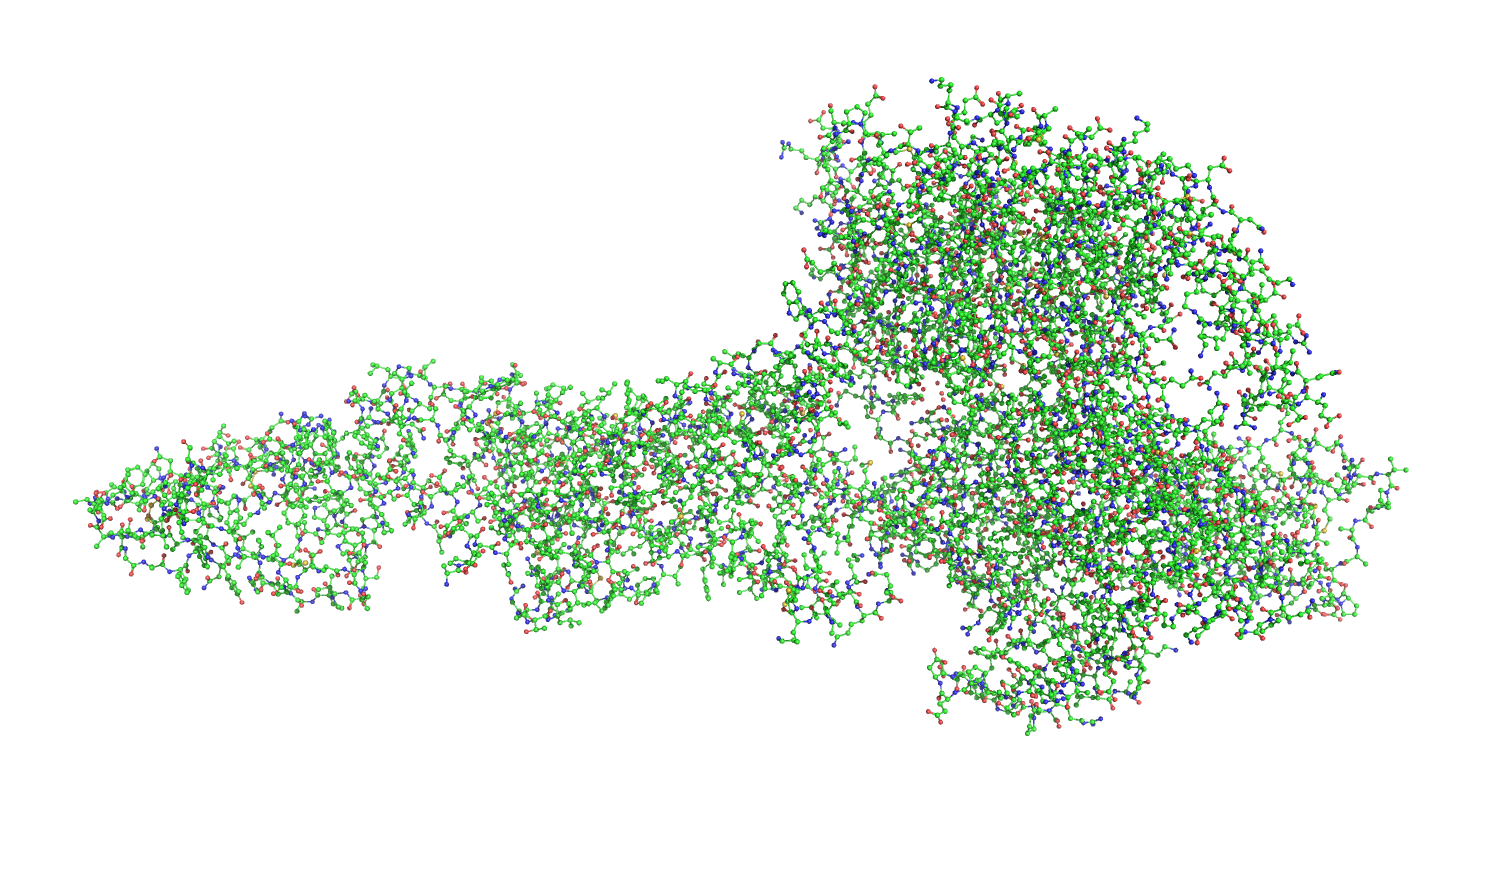
\includegraphics[width=0.85\textwidth]{prot.png}
	  \end{center}
  \end{frame}


\begin{frame}
    {Что такое белок?}{}
	\textbf{Белки}  — высокомолекулярные органические вещества, состоящие из соединённых в цепочку пептидной связью альфа-аминокислот.(wikipedia) \\
	\vspace{.5cm}
	\begin{center}
	\small%
	\chemfig[atom sep=2em]{-N(-[2]H)-C(-[2]H)(-[6]R_1)-C(=[2]O)-N(-[6]H)-C(-[6]H)(-[2]R_2)-C(=[6]O)-N(-[2]H)-C(-[2]H)(-[6]R_3)-C(=[2]O)-}\\
	\vspace{.5cm}
    \end{center}
	\textbf{Или:} белок это линейный полярный полимер, где мономерами является выборка из примерно 20 L-альфа-аминокислот. 

\end{frame}

\setchemfig{atom sep=2em, cram width=0.2em}

\begin{frame}
    {Что такое  L альфа-аминокислота?}{}
	\begin{center}
%\setatomsep{2.7em}\setcrambond{0.2em}{}{}%
 \chemfig{C(-[5]H)(-[2]H)(<[:-60]H)(<:[:-20]H)} \\
 \small
 атом углерода в $sp^3$ гибридизации имеет тетраэдрическое окружение\\
  \vspace{.5cm}
 \chemfig{C(-[5]NH)(-[7]CO)(<[:60]R_1)(<:[:120]H)}
 \hspace{1cm}
 \chemfig{C(-[5]NH)(-[7]CO)(<:[:60]R_1)(<[:120]H)}\\
 \vspace{.2cm}
 L-аминокислота \hspace{1cm} D-аминокислота \\
 \end{center}
% \chemfig{C(-[5]NH)(-[2]R_1)(<[:-60]CO)(<:[:-20]H)}
\end{frame}

\begin{frame}
    {Аминокислоты}
	\begin{center}
          \includegraphics[width=.9\textwidth]{Amino_Acids}
          %[height=.7\textheight]{Amino_Acids}
    \end{center}
  \end{frame}


\begin{frame}
    {Пептидная связь}
	\begin{center}
%		         \setlength{\fboxsep}{1pt}
%				            \fcolorbox{black}{white}{ 
%          \includegraphics[width=.8\textwidth]{pep1.eps}
  \begin{tikzpicture}[help lines/.style={thin,draw=black!50}]
%  \draw[help lines] (0,0) grid (8,4);    
   \node (2) at (4,2) {
   % \schemedebug{true}
     %\setatomsep{2.7em}\setcrambond{0.2em}{}{}%
     %\setbondstyle{line width=1pt}
     \chemfig{
         H_2N-[1](-[2]R_1)-[7]C(=[6]O)-[1,,,,white!40!blue,{line width=2pt}]N(-[2]H)-[7](-[6]R_2)-[1]C(=[2]O)-[7,,,,white!40!blue,{line width=2pt}]N(-[6]H)
         -[1](-[2]R_3)-[7]C(=[6]O)-[1]OH
         }
	  };
      \draw[orange] (1.5,1.8) ellipse (1.3cm and 2cm);
      \draw[orange] (3.7,2.3) ellipse (1.2cm and 2cm);
      \draw[orange] (5.9,1.8) ellipse (1.2cm and 2cm);
      \node (pep) at (4,-1) {Пептидные связи};
      \draw [->,white!40!blue,thick] (pep.north) -- (2.8,2);
      \draw [->,white!40!blue,thick] (pep.north) -- (4.8,2);
      %node[ellipse, minimum height=4cm,minimum width=2cm,draw] {};
  \end{tikzpicture}
 \end{center}
\end{frame}

\begin{frame}
    {Пептидная связь, таутомерия}
	\begin{center}
	 \schemestart
	 \small%
%		 \setatomsep{2em}%
%\setatomsep{2.7em}\setcrambond{0.2em}{}{}%
	 \chemfig{C(-[5])(<:[:60]H)(<[:120]R_1)-[7]C(=[6]O)-[1,,,,white!40!blue,{line width=1pt}]N(-[2]H)-[7]C(<:[:-60]R_2)(<[:-120]H)-[1] }%
	 \arrow{<=>}%
%\setatomsep{2.7em}\setcrambond{0.2em}{}{}%
	 \small\chemfig{C(-[5])(<:[:60]H)(<[:120]R_1)-[7]C(-[6]OH)=[1,,,,white!40!red,{line width=1pt}]N-[7]C(<:[:-60]R_2)(<[:-120]H)-[1] }%
	  \schemestop
    \end{center}
\end{frame}

\begin{frame}
{Пептидная связь, свойства}
	\begin{itemize}
		\item Пептидная связь прочнее, чем другие амиды
		\item Атомы пептидного звена ( C$_\alpha$-C-N- C$_\alpha$) лежат в одной плоскости
    \item Валентные углы у атомов С и N примерно равны $120^o$
		\item Вращение вокруг связи C-N затруднено
		\item Возможны cis- и trans-конфигурации; в белках преобладают trans
		\item Карбонильный кислород – хороший акцептор водорода
		\item Амидный азот – хороший донор водорода
		\end{itemize}
 \end{frame}

 \begin{frame}
{Вращения вокруг связей в остове белка}
	\begin{center}
%`\setatomsep{3.7em}\setcrambond{0.2em}{}{}%
	 \chemfig{C(-[5])(<:[:60]H)(<[:120]R_1)-[7]C(=[6]O)-[@{om}1]N
     (-[2]H)-[@{phi}7]C(<:[:-60]R_2)(<[:-120]H)-[@{psi}1]C(=[2]O)-[7]}%
 \chemmove{%
     \draw[-stealth,thick,white!40!red]
     (phi).. controls +(45:5mm) and +(-90:5mm).. node[above right]
     {$\boldsymbol{\phi}$}(phi);
     \draw[-stealth,thick,white!40!blue]
     (psi).. controls +(135:5mm) and +(-90:5mm).. node[below right]
     {$\boldsymbol{\psi}$}(psi);
     \draw[-stealth,thick,green!60!black]
     (om).. controls +(135:5mm) and +(-90:5mm).. node[above left]
     {$\boldsymbol{\omega}$}(om);
 }
	  \end{center}
  \end{frame}




  \begin{frame}
{Вращения вокруг связей в остове белка}
	\begin{center}
%\setatomsep{3.7em}\setcrambond{0.2em}{}{}%
	 \chemfig{C(-[5])(<:[:60]H)(<[:120]R_1)-[7]C(=[6]O)-[@{om}1]N
     (-[2]H)-[@{phi}7]C(<:[:-60]R_2)(<[:-120]H)-[@{psi}1]C(=[2]O)-[7]}%
 \chemmove{%
     \draw[-stealth,thick,white!40!red]
     (phi).. controls +(45:5mm) and +(-90:5mm).. node[above right]
     {$\boldsymbol{\phi}$}(phi);
     \draw[-stealth,thick,white!40!blue]
     (psi).. controls +(135:5mm) and +(-90:5mm).. node[below right]
     {$\boldsymbol{\psi}$}(psi);
     \draw[-stealth,thick,green!60!black]
     (om).. controls +(135:5mm) and +(-90:5mm).. node[above left]
     {$\boldsymbol{\omega}$}(om);
 }
	  \end{center}

 $ \begin{array}{l}  \phi\\ \psi  \end{array}  \Bigg \} $ теоретически могут быть: от –180$^0$ до +180$^0$ \\
 \vspace{.5cm}
	  а $\omega$ ?
  \end{frame}

  \begin{frame}
{Карта Рамачандрана}
	  даже в полиглициновой цепи существуют стерические ограничения
	\begin{center}
          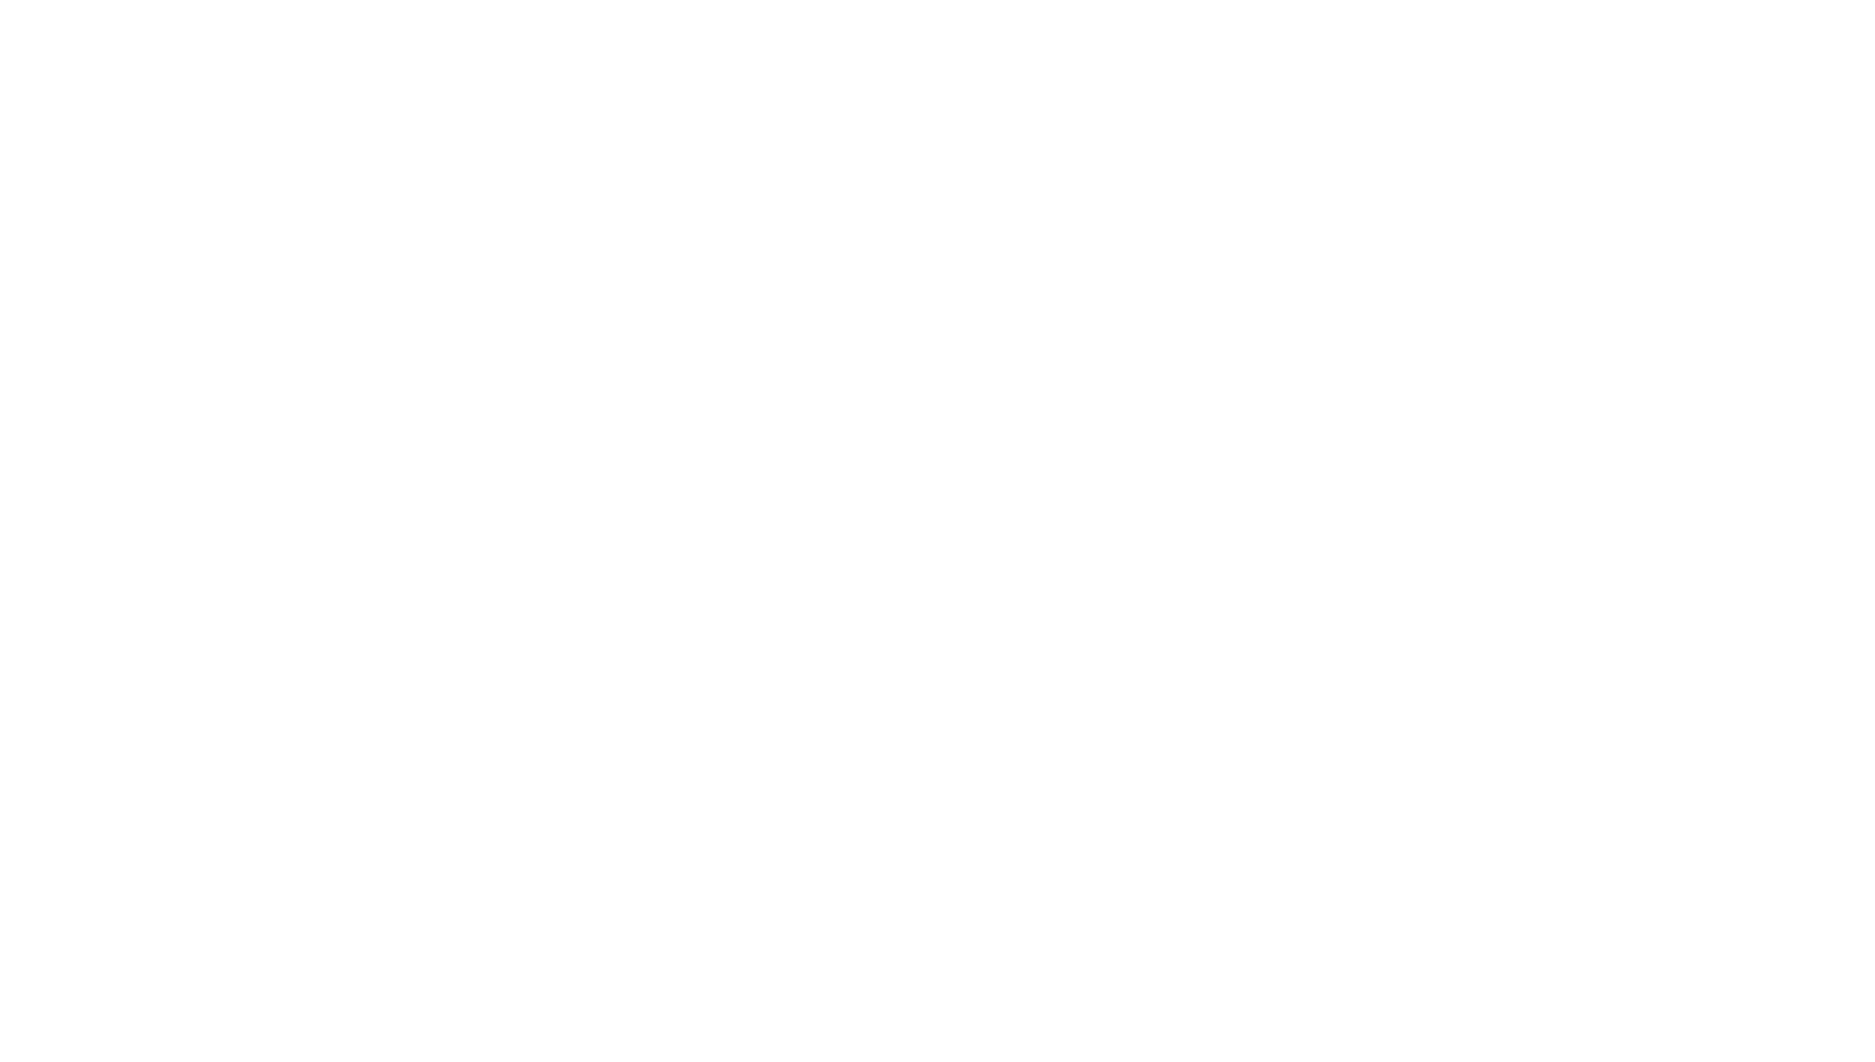
\includegraphics[width=0.75\textwidth]{ram_gly.png}
	  \end{center}
  \end{frame}
 
  \section{Уровни организации структуры белка}
  \begin{frame}
{Уровни организации структуры белка}
	  \begin{itemize}
		  \item Первичная структура
		  \item Вторичная структура
		  \item Укладка (fold)
		  \item Третичная структура
		  \item Четвертичная структура
		  \end{itemize}
	  \end{frame}

  \begin{frame}
{Первичная структура}
	  Первичная структура – это аминокислотная последовательность:\\
	  \vspace{.5cm}
	  Met-Ala-Gly-Trp-Ala-Val-Asp \ldots
  \end{frame}

  \begin{frame}
{Вторичная структура}
	  \begin{wrapfigure}{r}{2cm}
	  \includegraphics[width=2cm]{ab.png}\\
	  \includegraphics[width=2cm]{bturn.png}
      \end{wrapfigure}
	  \textbf{Вторичная структура белка} - это упорядоченные расположения атомов основной цепи полипептида, 	 безотносительно к типам боковых цепей (групп) и их конформациям.\\
	  \vspace{.5cm}
	  Если упорядоченность такова, что двугранные углы
	  одинаковы у всех остатков, то говорят о
	  регулярной вторичной структуре. Регулярными
	  вторичными структурами являются спирали и $\beta$–
	  структуры.\\
	  \vspace{.7cm}
	  Пример нерегулярной вторичной структуры 
	  $\beta$–поворот ($\beta$–изгиб, реверсивный поворот).
  \end{frame}


  \begin{frame}
{Регулярные вторичные структуры}
	\begin{center}
%		         \setlength{\fboxsep}{3pt}
%				            \fcolorbox{black}{white}{ 
          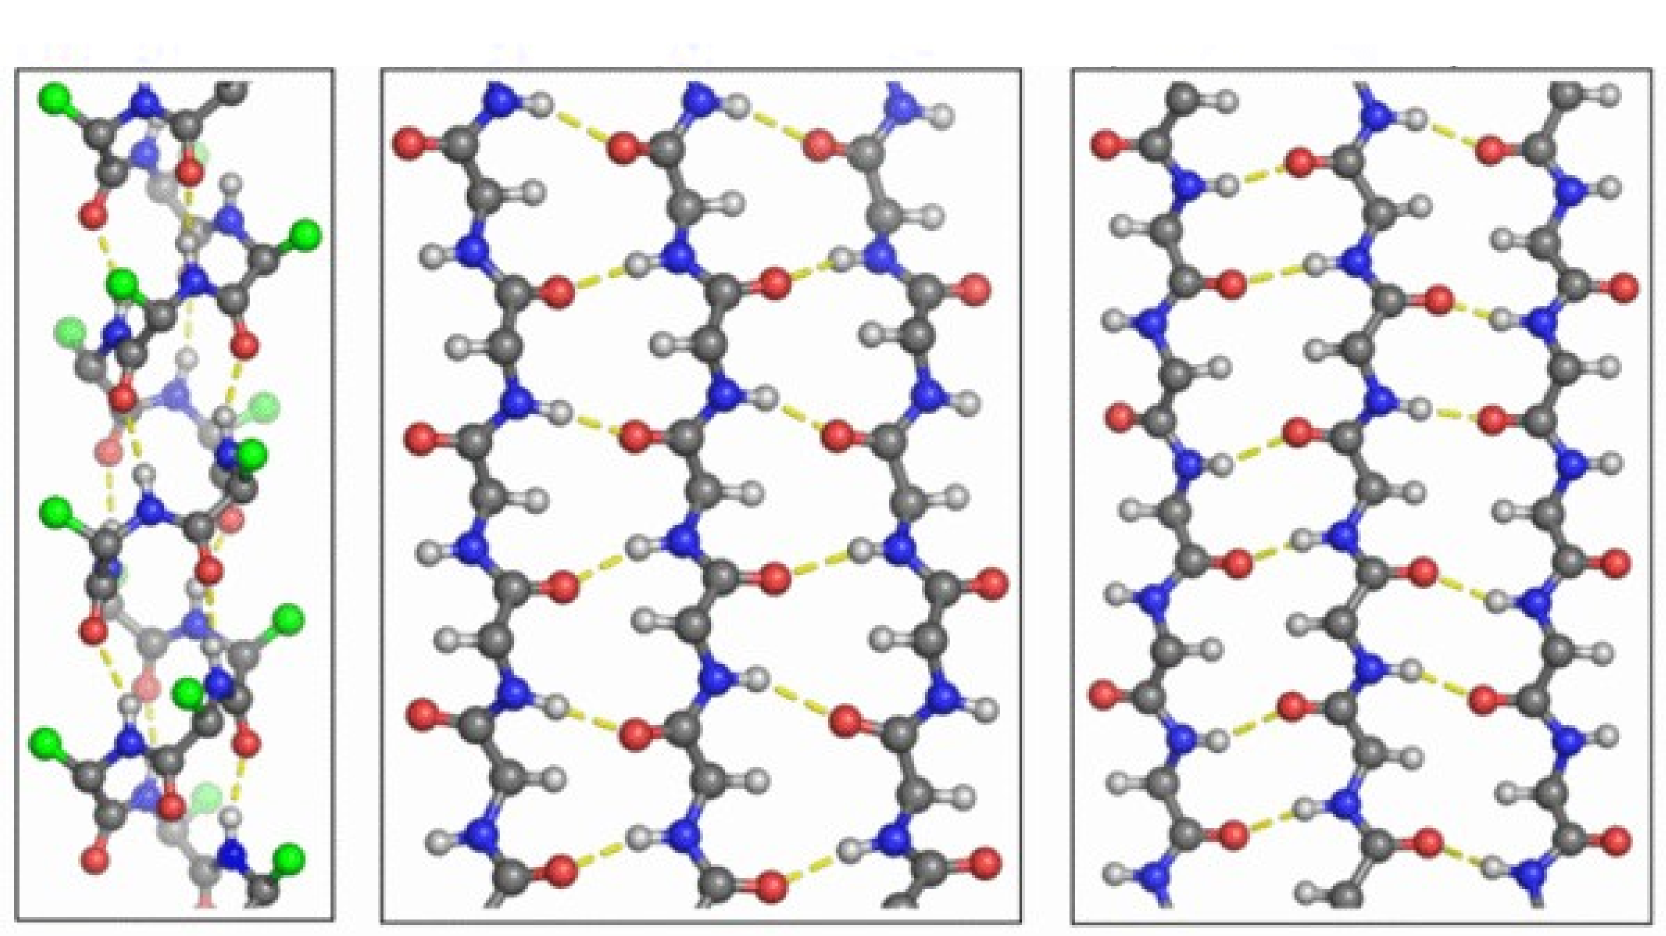
\includegraphics[width=0.8\textwidth]{ss.png}
%	  }
	  \end{center}
	\end{frame}

	\begin{frame}
{Укладка (fold)}
		Укладкой называют организацию в пространстве элементов регулярной вторичной структуры. \\
		Пример: $\alpha$ -спиральные белки\\
	\begin{center}
          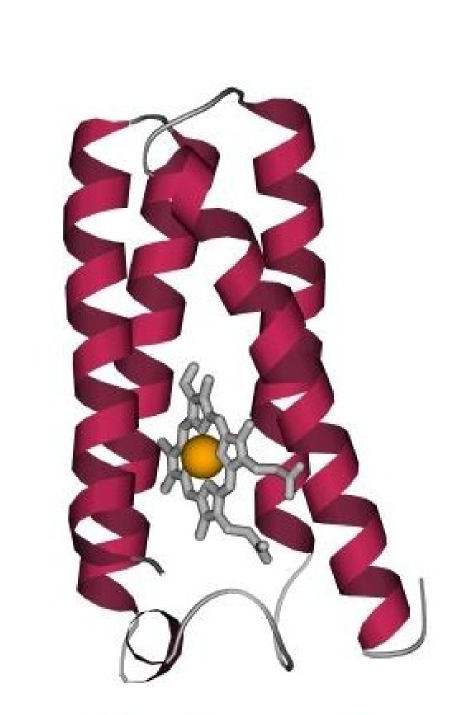
\includegraphics[width=0.2\textwidth]{ss1.png}
          
\includegraphics[width=0.2\textwidth]{ss2.png}
          \includegraphics[width=0.2\textwidth]{ss3.png}
	  \end{center}
	\end{frame}

\begin{frame}
{\texorpdfstring{$\beta$} - структурные белки}
	\begin{center}
		         %\setlength{\fboxsep}{0pt}
				  %          \fcolorbox{black}{white}{ 
								\begin{minipage}{\textwidth}
         % \includegraphics[width=0.5\textwidth]{b1.png}
         % \includegraphics[width=0.5\textwidth]{b2.png} \\
          \includegraphics[height=0.6\textheight]{b3.png}
          \includegraphics[height=0.6\textheight]{b4.png}
	  \end{minipage}
	  %}
	  \end{center}
	\end{frame}

	\begin{frame}
{Распределение в природе}
	\begin{center}
          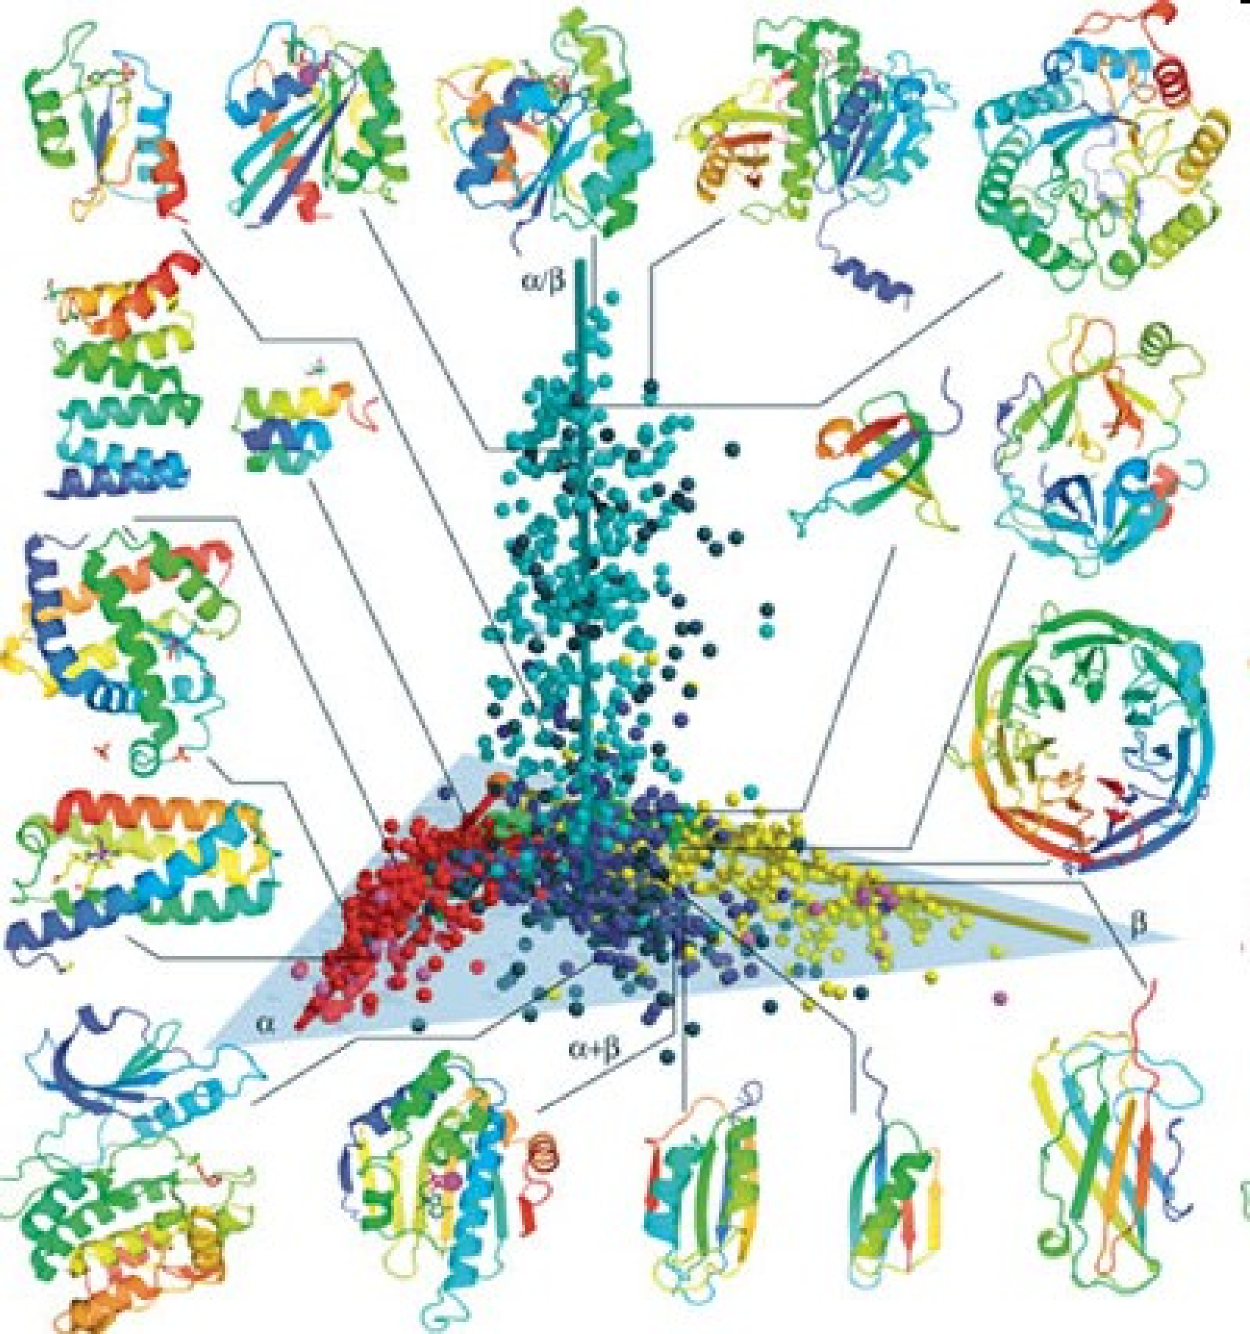
\includegraphics[width=0.4\textwidth]{scheme1.png}
	  \end{center}
	\end{frame}

	\begin{frame}
{Третичная структура}
		Третичной структурой называют расположение в пространстве всех атомов
		одной полипептидной цепи. \\
		Т.e. описание третичной структуры включает в себя:
		\begin{itemize}
			\item описание элементов вторичной структуры,
			\item описание типа укладки,
			\item описание структуры петель,
			\item описание конформаций боковых групп всех аминокислотных остатков.
			\end{itemize}
		\end{frame}
\section{Типы взаимодействий в белках}

\begin{frame}
{Вспомогательные взаимодействия: водородные связи}
	\begin{center}
        \chemfig{
            -[5]N-[7]C_\alpha(-[5]C(-[7])=[4]O)--[1]@{o1}O-H
            -[7,,,,dashed]@{o2}\Charge{120=\:,-120=\:}{O}=C(-[::60]\Charge{60=\-}{O})-[::-60]--[::-60]
        }
  \chemmove[dashed,white!40!red]{
  \draw[->] (o1) -- (o2)  node[below left] {3.5\AA\hspace{1cm}~};}

		%         \setlength{\fboxsep}{3pt}
	%			            \fcolorbox{black}{white}{ 
    %      \includegraphics[width=0.7\textwidth]{hbond.eps}
	%  }
	  \end{center}
  \end{frame}

\begin{frame}
{Ионные пары}
	\begin{center}
        \chemfig{
            --[1]--[7]@{o1}\chemabove{NH_3}{\oplus}
            -[:-90,1.5,,,draw=none,white!40!red]@{o3}\Charge{120=\:,-120=\:}{O}=[::90]C(-[::60]@{o2}O^{-})
            -[::-60]-[::60]-[::-60]
        }
  \chemmove[dashed,white!40!red]{
  \draw[->] (o1) -- (o2)  node[below left] {~};
  \draw[->] (o1) -- (o3)  node[below left] {3.1\AA\hspace{1cm}~};}
	  \end{center}
  \end{frame}

\begin{frame}
{Дисульфидные мостики характерны для секретируемых белков}
	\begin{center}
        \chemfig{
            -[5]N-[7]C_\alpha(-[5]C(-[7])=[4]O)--[1]S-[0,,,,yellow!60!black,
            thick]S-[7]
            -[0]C_\alpha(-[1])-[7]
        }
	  \end{center}
  \end{frame}

\begin{frame}
{Гидрофобные взаимодействия – главный 	фактор, заставляющий глобулу свертываться}
	\begin{center}
  \begin{tikzpicture}[help lines/.style={thin,draw=black!50}]
  %\draw[help lines] (0,0) grid (8,4);    
   \node (2) at (4,2) {
     \chemfig{
         (-[1,0.5,,,draw=none]-[1,2,,,decorate,decoration=snake]COO^{-})
         (-[2,0.5,,,draw=none]-[2,2,,,decorate,decoration=snake]COO^{-})
         (-[0,0.5,,,draw=none]-[0,2,,,decorate,decoration=snake]COO^{-})
         (-[7,0.5,,,draw=none]-[7,2,,,decorate,decoration=snake]COO^{-})
         (-[5,0.5,,,draw=none]-[5,2,,,decorate,decoration=snake]^{-}OOC)
         (-[3,0.5,,,draw=none]-[3,2,,,decorate,decoration=snake]^{-}OOC)
         (-[4,0.5,,,draw=none]-[4,2,,,decorate,decoration=snake]^{-}OOC)
         (-[6,0.5,,,draw=none]-[6,2,,,decorate,decoration=snake]COO^{-})
 }};
      \draw[orange] (4,2) ellipse (2cm and 2cm);
      \node (pep) at (5,0) {$\approx$ 4\AA};
 \end{tikzpicture}

	  \end{center}
  \end{frame}




\begin{frame}
{От четвертичной структуры к молекулярным машинам}
	\begin{center}
%		         \setlength{\fboxsep}{0pt}
%				            \fcolorbox{black}{white}{ 
          \includegraphics[height=0.6\textheight]{4s1.png}
          \includegraphics[height=0.6\textheight]{4s2.png}
%	  }
	  \end{center}
  \end{frame}
	



\section{Базы данных  и выравнивание}

\begin{frame}{UniProt Knowledgebase}
    UniProtKB – две базы аннотированных белковых последовательностей с общим форматом
записей.
\begin{itemize}
    \item \textbf{TrEMBL} (от Translated EMBL) – автоматическая база данных, содержащая, в основном,
формальные трансляции открытых рамок считывания, предсказанных в нуклеотидных последовательностях.
    \item \textbf{Swiss-Prot} (раньше была отдельным банком) – курируемая база данных. Кураторы выбирают
записи из TrEMBL, проверяют и дополняют их, переносят в Swiss-Prot.
\end{itemize}
\end{frame}

\begin{frame}{Рост числа записей в Swiss-Prot}
    \centering
    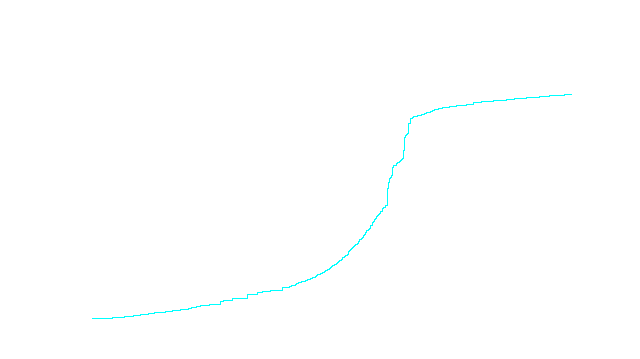
\includegraphics[height=0.9\textheight]{uniprot-stat1}
\end{frame}

\begin{frame}{Одна запись UniProtKB}
    \begin{itemize}
        \item     Одна запись – все продукты одного гена из организмов одного вида. Известные изоформы,
полиморфизмы и т.д. указывают в аннотации записей.
        \item Изоформы указаны в полях СС (подраздел "Alternative products") и FT (конкретные участки
различий), полиморфизмы указывают в поле FT.
    \item Правило не строгое, из него есть исключения. Например, если для гена известно множество
изоформ, сильно отличающихся по последовательности и функциям, то для них создадут несколько записей
    \end{itemize}
\end{frame}

\begin{frame}[fragile]{Таблица локальных особенностей (Feature table, FT)}
Имеет строгий формат, список и описание всех возможных ключей доступно на сайте UniProt.
\begin{multicols}{2}
    \tiny
    \begin{verbatim}
FT CHAIN 1..188
FT /note="Isochorismatase family protein YecD"
FT /id="PRO_0000201831"
FT HELIX 6..8
FT /evidence="ECO:0000244|PDB:1J2R"
FT STRAND 9..14
FT /evidence="ECO:0000244|PDB:1J2R"
FT REGION 5..34
FT /note="Interaction with RNase E"
FT ACT_SITE 209
FT /note="Proton donor"
FT /evidence="ECO:0000255|HAMAP-Rule:MF_00318,
FT ECO:0000269|PubMed:15003462"
FT METAL 246
FT /note="Magnesium"
FT /evidence="ECO:0000269|PubMed:11676541,
FT ECO:0000269|PubMed:16516921"
FT BINDING 159
FT /note="Substrate"
FT /evidence="ECO:0000255|HAMAP-Rule:MF_00318"
FT MOD_RES 257
FT /note="N6-acetyllysine"
FT /evidence="ECO:0000269|PubMed:18723842"
FT CONFLICT 180..188
FT /note="SVEEILNAL -> TWKRSSTRYDLHRSTAMVAS (in Ref. 1)"
\end{verbatim}
    \columnbreak
    \normalsize
    вторичная структура\\
    \vspace{1cm}
сайты связывания\\
    \vspace{1cm}
модифицированные остатки\\
    \vspace{1cm}
разночтения в
последовательности\\
    \vspace{1cm}
и т.д.
\end{multicols}
%\begin{tikzpicture}
%    \node (A) {}
%\end{tikzpicture}
\end{frame}

\begin{frame}{Выравнивание}
    \centering
    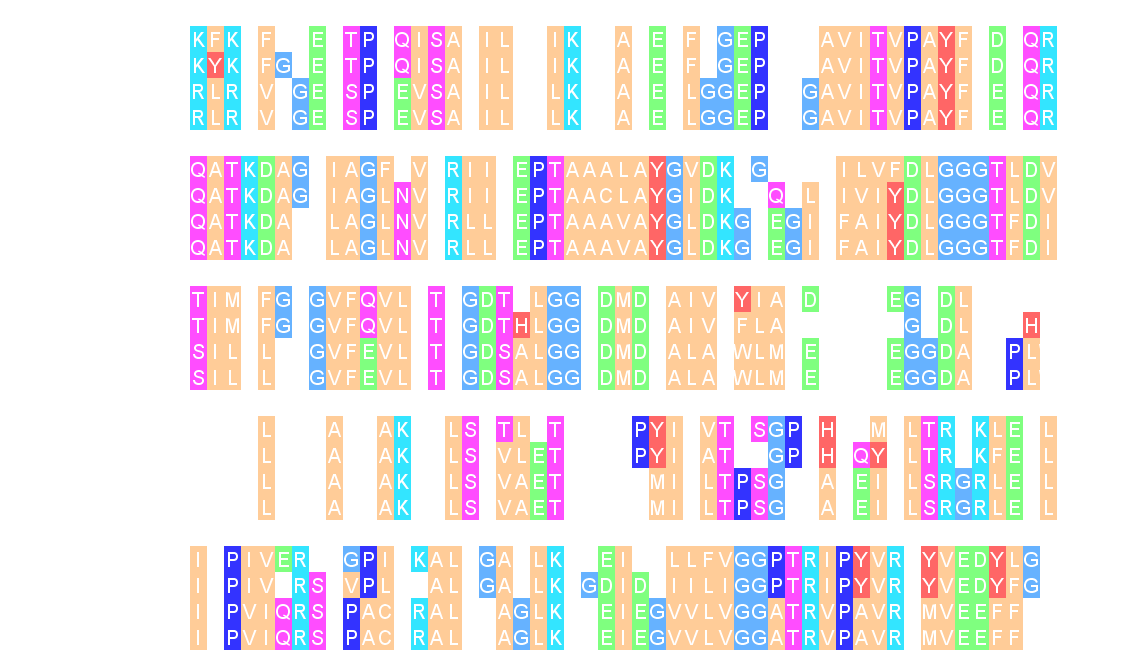
\includegraphics[height=0.9\textheight]{alighment}

\end{frame}


\section{Общие рассуждения}
\begin{frame}{Как устроено вещество?}
   \begin{itemize}
     \item Первые шаги к пониманию того, что вещество состоит из маленьких элементов сделал Лукреций, давно. 
    \vspace{0.2cm}
     \item Первые эксперименты по установлению структуры  были проведены только в начале 20 века
    \vspace{0.2cm}
     \item Появились специальные молекулярные наборы из шариков и палочек
    \vspace{0.2cm}
     \item Правильное использование химической информации позволило строить первые модели,
         очень похожие на результаты РСА.
    \end{itemize}
\end{frame}

\begin{frame}{Как это работает?}
    \centering
    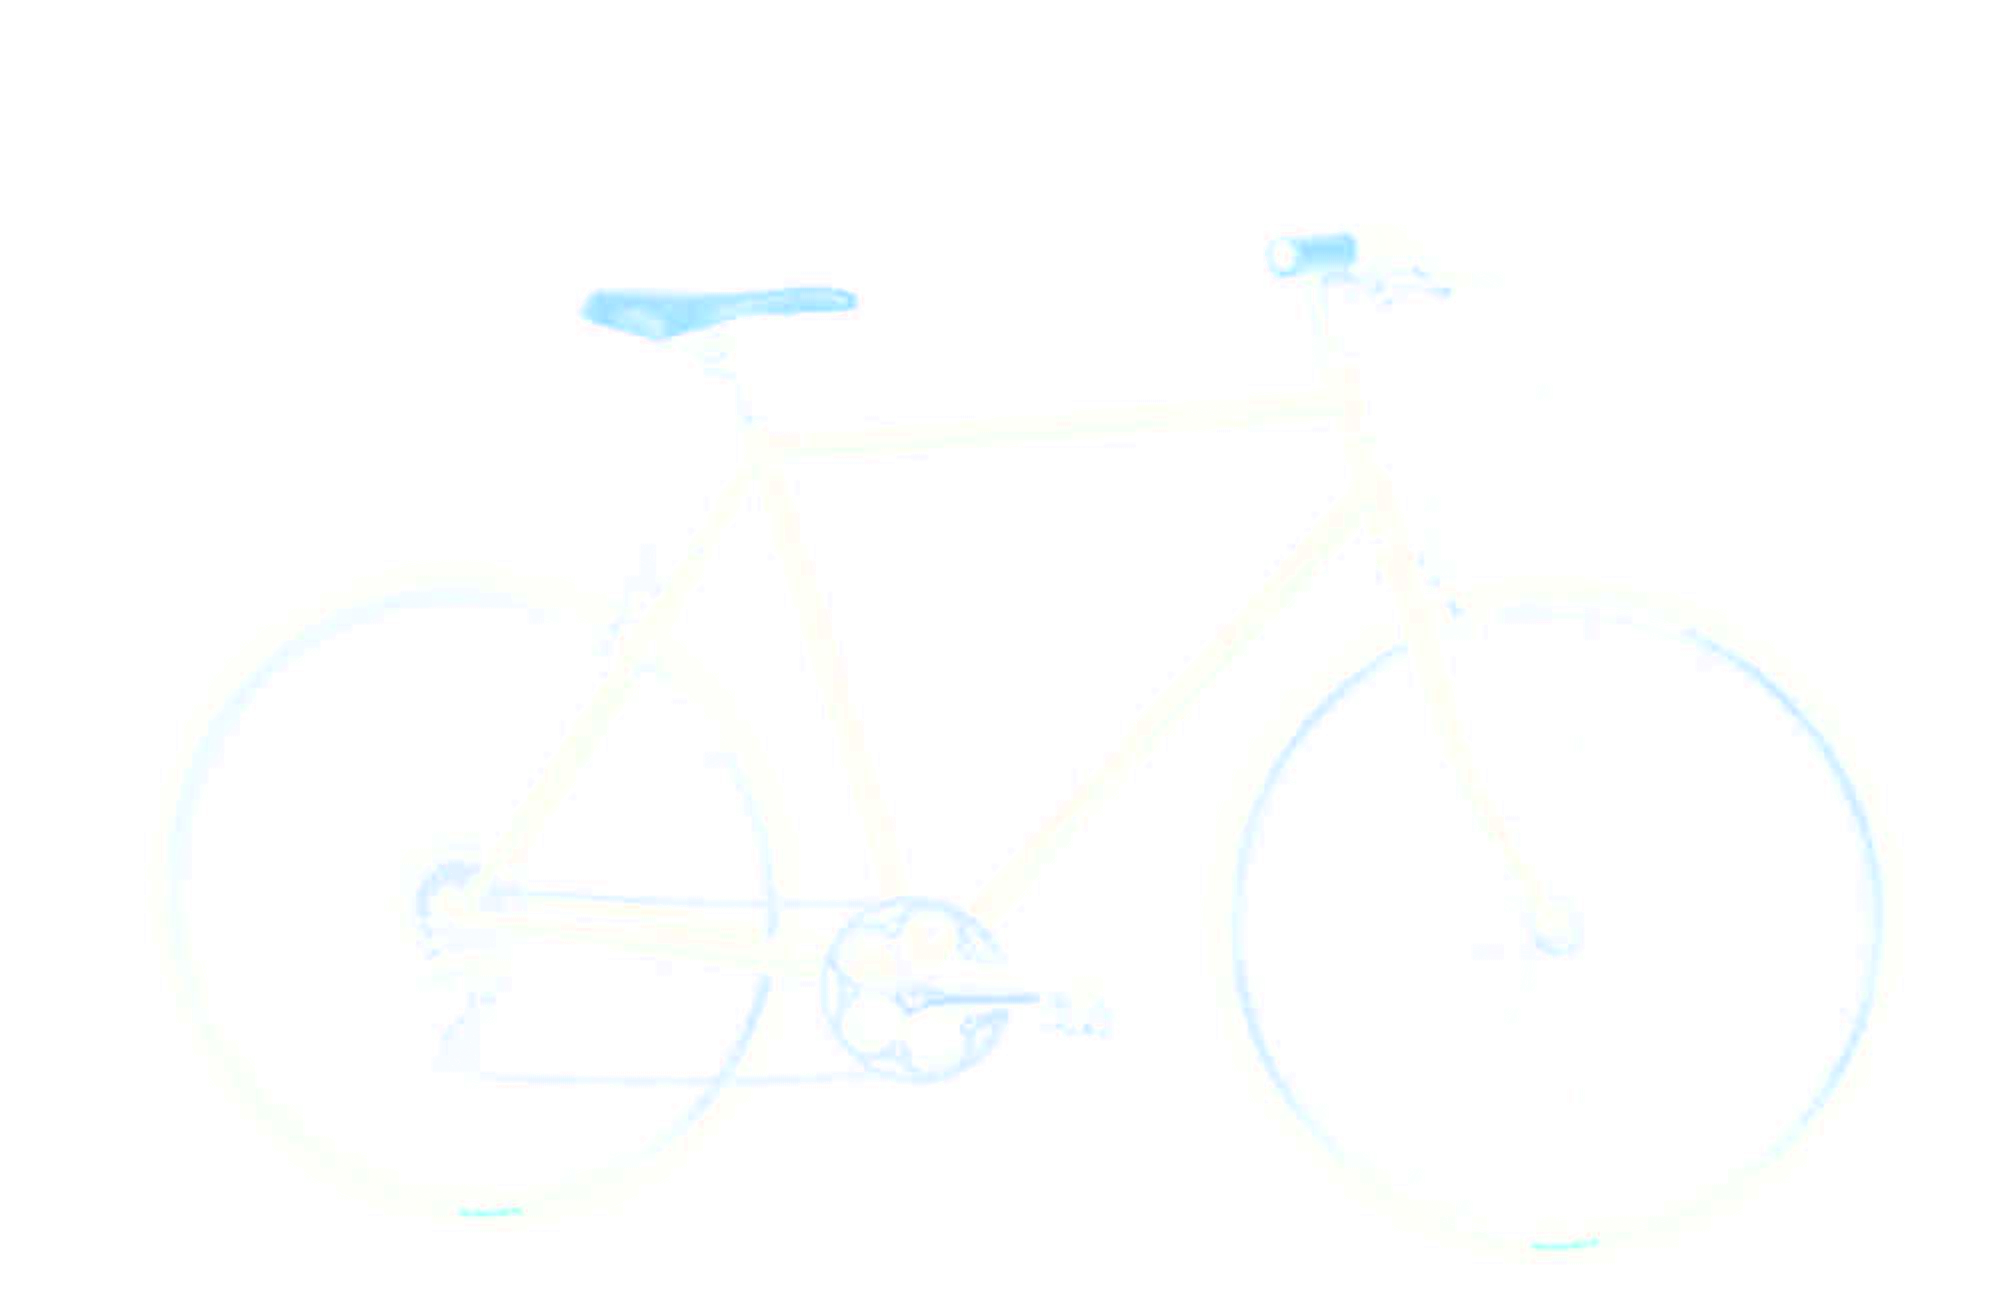
\includegraphics[height=0.9\textheight]{bicycle}
\end{frame}

\begin{frame}{Для чего нужны модели?}
  \begin{itemize}
   \item
Упрощение сложного объекта до анализа только той части которая предполагаемо является объектом интереса.\\
    \vspace{0.5cm}
   \item
Модель является иллюстрацией для дедуктивного анализа очень сложных или многочисленных явлений.\\
    \vspace{0.5cm}
   \item
Часто модели отражают  реальность не полностью, но моделируемой точности бывает достаточно для понимания рассматриваемой системы.
\end{itemize}
\end{frame}


\begin{frame}{Финальный этап: Дизайн}
    Моделирование структуры, определение свойств это шаги к самому важному этапу : \\
    \vspace{0.5cm}
    \textbf{
    дизайну или проектированию нового с заданными свойствами.}
\end{frame}

\begin{frame}{Маcштабы в моделировании}
    %      \includegraphics[width=0.9\textwidth]{scope}
    \centering
    \begin{tikzpicture}[every node/.style={scale=0.9}]
    \begin{axis}
        [
        ,width=0.8\textwidth
        ,height=0.8\textheight
        ,xlabel={Размер}
        ,ylabel={Время}
        %,xtick=data,
        ,xtick={0,1,...,4}
        ,xticklabels={'',A,нм,мкм,мм,м}
        ,yticklabels={'',фс,пс,нс,мкс,мс,с,часы, годы}
        ]
        %\addplot+[sharp plot] coordinates   {(0,18.26) (1,21.47) (2,24.58) (3,24.95)};
    \end{axis}
    \draw[draw=black,fill=red!10!black] (0,0) rectangle ++(2.5,1) node[pos=.5] {Электроны};
    \draw[draw=black,fill=yellow!10!black] (1.5,0.8) rectangle ++(2.5,1) node[pos=.5] {Атомы};
    \draw[draw=black,fill=green!10!black] (3,1.6) rectangle ++(3,2) node[pos=.5] {Группы атомов};
    \draw[draw=black,fill=blue!10!black] (5.5,3.4) rectangle ++(4,3) node[pos=.5] {Cплошные среды};
%\draw (0,0) rectangle (2,1) node[pos=.5] {КМ};
%\draw (1.5,1) rectangle (2,1) node[pos=.5] {MМ};
\end{tikzpicture}
\end{frame}

\begin{frame}{Компьютер}
    \begin{itemize}
     \item Формально для решения задач моделирования компьютер не является обязательным элементом
    \vspace{0.2cm}
     \item Быстрый компьютер значительно увеличивает точность и широту исследования, и следовательно достоверность моделирования.
    \vspace{0.2cm}
     \item Количество вычислений отражает степень исследования конформационного
         пространства
    \end{itemize}
\end{frame}

\begin{frame}{Компьютер и программы}
    Those programs \textbf{always provide a result}, the evaluation of which is at liberty of the user. The programs 
    \textbf{tend stubbornly} to calculate \textbf{every absurd application} and present a result-not only a number, but also a graph and
    represent a further instrument of seduction for the uncritical use of algorithms. 
\end{frame}





	




\section{Введение}

\begin{frame}{Визуализация с PyMol}
	\begin{center}
          \includegraphics[height=0.75\textheight]{natures}
	  \end{center}
  \end{frame}

\begin{frame}{Для чего нужен PyMol}
	\begin{itemize}
	\item Визуализация pdb и прочих файлов с координатами атомов
	\item Изготовление высококачественных изображений
	\item Начальное редактирование структур
	\end{itemize}
\end{frame}

\begin{frame}{Системные требования}
	\textbf{Компьютер:} чем мощнее процессор и чем больше памяти, тем лучше\\
	\textbf{3D монитор} не обязателен, но поддерживается \\
	\textbf{Операционная система}: любая, под Linux проще установить, и он лучше работает с памятью.
\end{frame}

\begin{frame}{Как установить?}
	\begin{itemize}
		\item Компиляция из исходников:   http://pymol.svn.sourceforge.net/
		\item Установка бинарных пакетов в Ubuntu Linux: sudo apt-get install pymol
		\item Установка c Conda: conda install -c schrodinger pymol \\ 
		или  conda install -c conda-forge pymol-open-source
	   \end{itemize}
\end{frame}

\begin{frame}{PyMol - это GPL программа?}
	Да, PyMol это GPL-программа;
	\begin{itemize}
		\item исходный код доступен на sourceforge.net
		\item Бинарные пакеты для windows стоят денег и продаются: http://pymol.org/academic.html
		\item Бинарные пакеты для Linux собираются майтенерами
		\end{itemize}
	\end{frame}


  
  \section{Визуализация c PyMol}



  \begin{frame}{Меню объекта/выборки}
	\begin{center}
          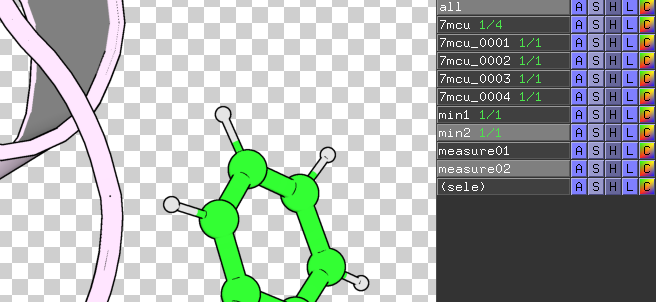
\includegraphics[height=0.7\textheight]{pymol-ashl}
	  \end{center}
  \end{frame}


\section{Selections} 
\begin{frame}{Выборки}
	\begin{itemize}
		\item Можно задать с помощью кликов мыши, удерживая SHIFT
		\item Удобнее писать выражения в командной строке
		\end{itemize}

	Например:
	\textit{Select backbone, name ca+c+n }
\end{frame}

\begin{frame}{Операторы множеств}
	\begin{itemize}
		\item Логические операторы AND, OR,  NOT\\
					Операция OR может быть записана как ",". \\
				{ \tiny
					Упражнение: Документ PDB содержит описание структуры, состоящей из белка,
					фрагмента ДНК и молекул воды. Что получится, если задать следующие
				команды ?}\\
				\textit{
					select protein or dna \\
					select protein and dna\\
				select not water}
			\item Оператор WITHIN(...) \\
				\textit{
					select all within 3.5 of resi 20\\
				select s1, (byres n. ca) within 3.5 of resn LIG}
	\end{itemize}
\end{frame}

			 \begin{frame}[fragile]
				 \frametitle{Help selections}
{\tiny
	\hspace{0.5cm}	Длинное \hspace{2cm}Короткое
\begin{verbatim}
 name <atom names>           n. <atom names>
 resn <residue names>        r. <residue names>
 resi <residue identifiers>  i. <residue identifiers>
 chain <chain ID>            c. <chain identifiers>
 id <original-index>
 hydrogen                    h.
 all                         *
 visible                     v.
 hetatm
 byres <selection>           br. <selection>
 byobj <selection>           bo. <selection>
 around <distance>           a. <distance>
 expand <distance>           e. <distance>
 in <selection>
 like <selection>            l. <selection>

 <selection> within <distance> of <selection>
 <selection> w. <distance> of <selection> 
\end{verbatim}
}

Актуальное:\\
https://pymolwiki.org/index.php/Selection\_Algebra

\end{frame}

 \begin{frame}{Примеры выборок}
sel=select
    \begin{itemize}
   \item sel s1, n. ca and c. A : все атомы СА в цепи А
   \item sel s2, n. ca and (c. A or c. B) : атомы СА цепей А и В
   \item sel s3, resn GLU and resi 100 : остаток 100 если он GLU
   \item sel s4, resi 100-120+130 : атомы остатков 100-120 и 130
   \item sel s5, byres( name CG) : атомы остатков где есть CG
    \end{itemize}
\end{frame}

\begin{frame}{Иерархическое определение выборки}
		\begin{columns}
		\column{0.6\textwidth}
		Легко увидеть иерархию правым кликом по атому
		\column{0.4\textwidth}
		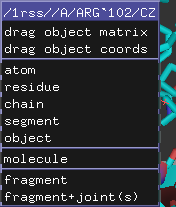
\includegraphics[height=0.3\textheight]{iearch.png}
		\end{columns}
		\textit{sel s1, a/102/cz}  : атом cz в остатке 102 \\
		\textit{sel s2, 100-120/N and c. A} : атомы N  в остатках 100-120 цепи а\\
		\textit{sel s3, a/100+120/} : все атомы остатков 100 и 120 в цепи А\\
\end{frame}

        
\begin{frame}{Трассировка лучей, команда ray }
	\small
	Подробно: \url{http://www.pymolwiki.org/index.php/Ray} \\
	\begin{columns}
		\column{0.3\textwidth}
		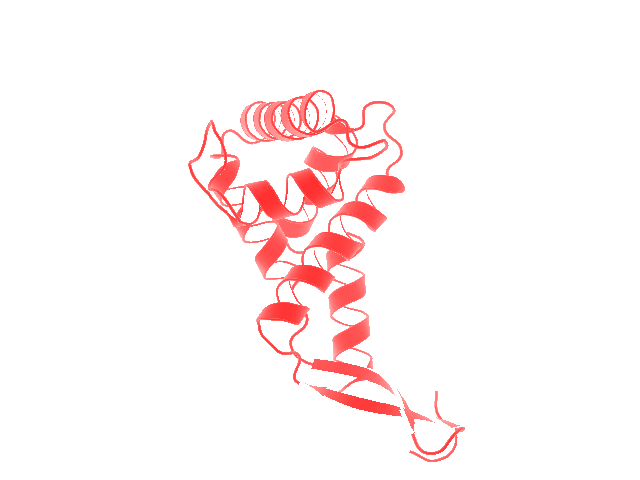
\includegraphics[height=0.3\textheight]{r1.png} \\
		No ray
		\column{0.3\textwidth}
		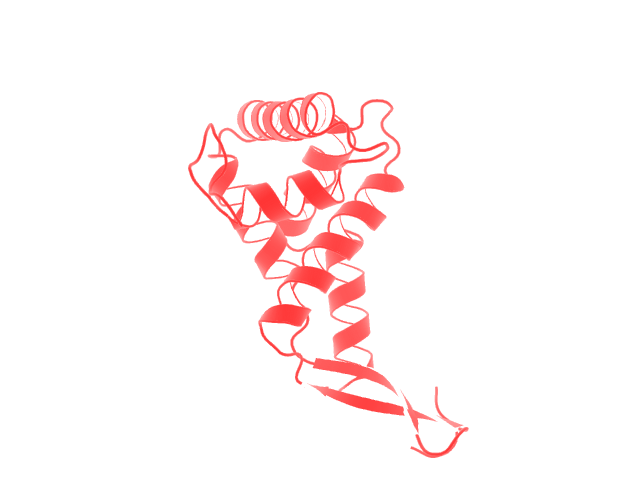
\includegraphics[height=0.3\textheight]{r2.png} \\
		ray\_trace\_mode,0
		\column{0.3\textwidth}
		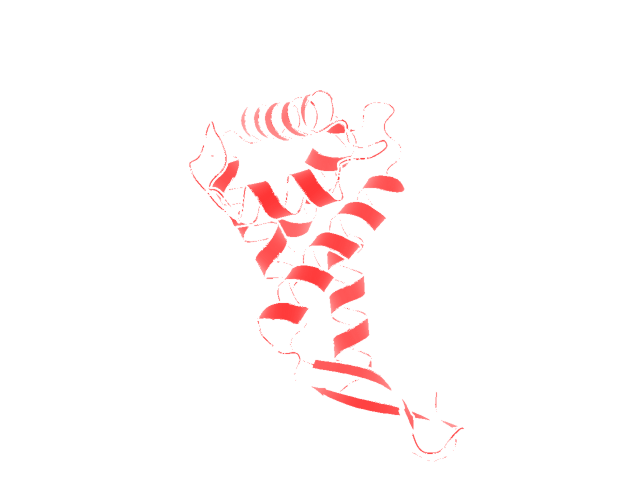
\includegraphics[height=0.3\textheight]{r3.png} \\
		ray\_trace\_mode,1
	\end{columns} 
	\begin{columns}
		\column{0.3\textwidth}
		
\includegraphics[height=0.3\textheight]{r4.png} \\
		ray\_trace\_mode,2
		\column{0.3\textwidth}
		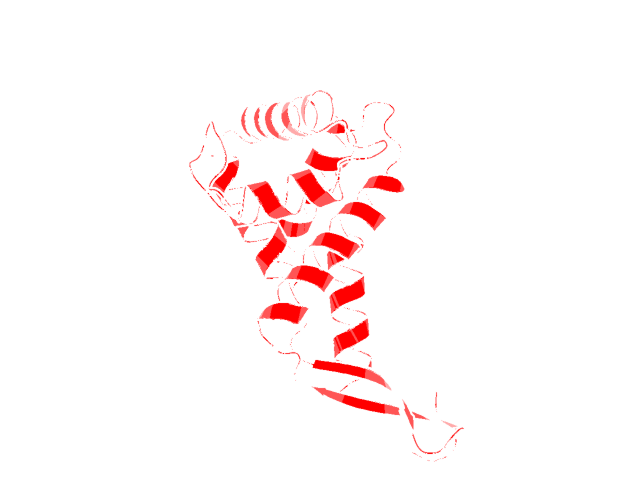
\includegraphics[height=0.3\textheight]{r5.png} \\
		ray\_trace\_mode,3
	\end{columns}
\end{frame}

\begin{frame}[plain]
	\centering
	\includegraphicsfs{coord-zn}
\end{frame}

\begin{frame}{Настройки изображения}
	\url{http://www.pymolwiki.org/index.php/Category:Settings}
	\begin{itemize}
		\item PyMol содержит порядка 600 настроек
		\item Не все документированы
		\item Большинство интуитивно понятны
		\item Настройки доступны через меню или в командной строке набрать: \\
			\textit{set {первые буквы имени опции} и клавиша tab для достроения}
	\end{itemize}
\end{frame}

\begin{frame}{Примеры}
	\small
	\#initial setup\\
	\textcolor{blue!40!white}{viewport 600, 600} --- размер графического окна\\
	\textcolor{blue!40!white}{set auto\_zoom, off} --- не приближать новые объекты\\
	\textcolor{blue!40!white}{set auto\_show\_lines, off} --- не показывать линии автоматически\\
	\textcolor{blue!40!white}{set auto\_show\_selections, off} --- не показывать выборку автоматически\\
	\#cartoon parameters\\
	\textcolor{blue!40!white}{set cartoon\_fancy\_helices,1} --- изменение вида спиралей\\
	\textcolor{blue!40!white}{set cartoon\_highlight\_color, grey60} ---цвет внутренней стороны спиралей\\
	\textcolor{blue!40!white}{set cartoon\_dumbbell\_length,1.0} ---ширина ленты в спирали\\
	\textcolor{blue!40!white}{set cartoon\_rect\_length,1.40000} --- ширина ленты в бета\\
	\textcolor{blue!40!white}{set cartoon\_loop\_radius,0.3} --- толщина неструкт. участка\\ 
	\textcolor{blue!40!white}{set cartoon\_smooth\_loops=0} --- без сглаживания\\
\end{frame}

\begin{frame}[fragile]{\$HOME/.pymolrc}
\centering
\begin{lstlisting}
set sphere_scale,0.2
set async_builds, 1
set ribbon_width, 8
set antialias, 2
\end{lstlisting}
\end{frame}

\begin{frame}[fragile]{\$HOME/.pymolrc.py}
\centering
\begin{lstlisting}[language=Python]
from pymol import cmd
from pymol import stored

@cmd.extend
def superall(target):
    seleobjs = cmd.get_object_list('all')
    for o in seleobjs:
        if o != target:
            cmd.super(o,target)
            print(o)
\end{lstlisting}

\end{frame}

\section{Анимация}

\begin{frame}{Анимация в PyMol}
\small Если структура содержит более чем одну модель, то в PyMol можно
            анимировать движение молекулы переходом от одной модели к другой\\
\centering
 \inlineMovie[loop&autostart]{../../avi/nuc_mov_small.avi}{nuc_mov_small}{height=0.7\textheight}
\end{frame}


	\begin{frame}{Пример}
		\begin{itemize}
			\item Action->Preset->Technical (viewer gui)
			\item Scene->Store->F1
			\item zoom i. 90   \# увеличение остатка 90
			\item Scene->Store->F2
			\item Movie->Program->Scene Loop->Y-Rock->4 Seconds Each
			\item File-> Save movie
			\end{itemize}
		\end{frame}

		\begin{frame}{Результат}
          \begin{center} 
 \inlineMovie[loop&autostart]{../../avi/m2.mpg}{m2}{height=0.9\textheight}
          \end{center}
	  \end{frame}

	  \begin{frame}{Анимация, терминология}
		  \begin{itemize}
			  \item Объект и выборка : смотри выше
			  \item states: конформация или набор координат
			  \item scene: позиция камеры и отображение
			  \item frames: это кадры в анимации, содержит state и scene
			  \end{itemize}
			  \begin{center}
			  Movie panel: \hspace{.5cm}
          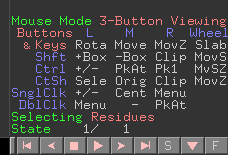
\includegraphics[width=0.2\textwidth]{an1.png}
	  \end{center}
	  \end{frame}

	  \begin{frame}{Анимация, команды}
		  \textcolor{blue!40!white}{mset 1 -55} : задать анимацию от 1 до 55 state на 55 кадров (frames) \\
		  \textcolor{blue!40!white}{mset 1 x90} : задать анимацию первого state от 1 до 90 кадров\\
		  \textcolor{blue!40!white}{mset 1 x30 1 -15 15 x30 15 -1 }: первые 30 кадров state 1, следующие 15 кадров это состояния 1-15, следующие 30 кадров состояние 15, следующие 15 кадров состояния от 15 до 1
	  \end{frame}

	  \begin{frame}{Анимация, команды}
			  mview : команда для создания ключевых точек \\
				  Пример :
		  \begin{itemize}
			  \item \textcolor{blue!40!white}{mset 1 x100}
			  \item \textcolor{blue!40!white}{frag leu}  \# создаём LEU
			  \item \textcolor{blue!40!white}{orient}    \# ориентируем его 
			  \item \textcolor{blue!40!white}{mview store} \# запоминаем ключевую точку
			  \item \textcolor{blue!40!white}{frame 100} \# переходим в кадр 100
			  \item \textcolor{blue!40!white}{zoom ID 10} \#  увеличиваем атом №10
			  \item \textcolor{blue!40!white}{mview store} \# запоминаем ключевую точку
			  \item \textcolor{blue!40!white}{mview reinterpolate} \# делаем интерполяцию
			  \end{itemize}
		  \end{frame}
		  
		  \begin{frame}{Результат mview}
          \begin{center} 
 \inlineMovie[loop&autostart]{../../avi/m4.mpg}{m4}{height=0.9\textheight}
          \end{center}
	  \end{frame}

	  \begin{frame}{Дополнительные команды}
		  \begin{itemize}
			  \item \textcolor{blue!40!white}{mmatrix} : устанавливает вид для первого кадра
			  \item \textcolor{blue!40!white}{util.mrock} : покачивание сцены на определённый угол 
			  \item \textcolor{blue!40!white}{util.mrock(start, finish, angle, phase, loop-flag) }
			  \item \textcolor{blue!40!white}{util.mroll} : вращение вокруг оси Y
			  \item \textcolor{blue!40!white}{util.mroll(start, finish, loop-flag)}
			  \item \textcolor{blue!40!white}{mdo} : (устарело) запуск какой-либо команды в заданном кадре
		   \end{itemize}
        Актульная информация:\\
        \textbf{https://pymolwiki.org/index.php/MovieSchool}

\end{frame}

	   \begin{frame}{Сохранение анимации}
		   \textbf{Старый путь: }\\
		   \textcolor{blue!40!white}{  set ray\_trace\_frames,1}\\
		   \textcolor{blue!40!white}{mpng mymovie}\\
		    Нужны программы avidemux, Virtual Dub, mencoder для того, чтобы собрать ролик с нужным сжатием (кодек)\\

			\textbf{Новый путь: File->Save movie }; есть недостаток, старый офис понимает только avi с определённым кодеком
		\end{frame}

		\section{Моделирование и редактирование в PyMol }

		\begin{frame}{Моделирование и редактирование в PyMol}
			\begin{itemize}
				\item Можно перемещать объекты и сохранять их новые координаты
				\item	Можно рассчитать вторичную структуру
				\item	Можно менять координаты отдельных атомов
				\item	Можно вносить мутации в белок (но не НК)
				\item	Можно конвертировать L->D аминокислоты
				\item	Можно добавлять протоны
				\item	Можно выравнивать в пространстве молекулы
				\item	Можно добавлять некоторые фрагменты из библиотеки и собственные
			\end{itemize}
		\end{frame}

		\begin{frame}{Перемещение объектов}
			Рекомендуемый порядок действий:\\
			\begin{itemize}
				\item \textcolor{blue!40!white}{set retain\_order} \# надо сохранить порядок атомов
				\item \textcolor{blue!40!white}{create newobj, sele} \# создаём новый объект, страховка
				\item \textcolor{blue!40!white}{translate [0,10,0], newobj} \# перемещаем
				\item \textcolor{blue!40!white}{rotate x,90,newobj} \# вращаем
				\item \textcolor{blue!40!white}{save newfile.pdb, newobj}
			\end{itemize}
			Операции по перемещению и вращению можно делать мышкой в режиме editing
		\end{frame}

		\begin{frame}{Изменение координат отдельных  атомов и объектов}

			\textcolor{blue!40!white}{alter\_state 1,(pdb1cse),x=x-10.0}\\
			Или 
			\textcolor{blue!40!white}{translate [0,10,0], A/100/NZ}

		\end{frame}

		\begin{frame}{Удаление связей,но не атомов}
			\begin{itemize}
				\item Выберите первый атом, ctrl+middle cliсk, выберите второй атом, ctrl+middle click

				\item И unbond или ctrl+D
			\end{itemize}

				\textbf{ Внимание! Координаты атомов не меняются, только исчезает изображение связи}
			
		\end{frame}

	\begin{frame}{Мутация аминокислот}
			\begin{itemize}
				\item Запустите wizard->mutagenesis 
				\item Выберите аминокислоту для мутации
				\item Справа выберите, на что мутировать
				\item Выберите ротамер с помощью управления movie
				\item Закончите процедуру с Apply
			\end{itemize}
	\end{frame}

     \begin{frame}{Добавление протонов}
			Работает с молекулами, т.е. объектами\\

			\textcolor{blue!40!white}{сreate gln, A/101/}\\
			\textcolor{blue!40!white}{h\_add gln}\\
			Или через меню action объекта.\\
			
			Есть вероятность, что протоны будут добавлены неверно, 
            если PyMol неправильно угадал валентность тяжёлых атомов.

	\end{frame}

	\begin{frame}{Суперпозиция в пространстве}
			Задача достаточно нетривиальная, и есть разные пути:\\

			Белки:\\
			 \textcolor{blue!40!white}{align, super, fit}\\
			Другое:\\
			 \textcolor{blue!40!white}{pair\_fit }\\
			Желательно указывать родственные атомы в молекулах\\
			 \textcolor{blue!40!white}{pair\_fit ( trna10 and resid 10:15 and name P ), ( ref4 and resid 10:15 and name P ) }
	 \end{frame}
		 
	\begin{frame}{Добавление органических фрагментов или а.к.}
			\begin{itemize}
				\item С помощью ctrl+middle click выделите шариком атом, к которому будет присоединяться фрагмент
				\item В меню Build выберите нужный фрагмент
				\item С помощью ctrl+left click выберите торсионный угол\\
					Или \\
				\item Создайте свою молекулу (ChemSketch)
				\item Сохраните как pkl в  <pymol\_path>/data/chempy/fragments
				\item \textcolor{blue!40!white}{editor.attach\_fragment('pk1','my\_fragment\_name',11,0)}\\
					  11 - это номер атома в фрагменте для связи
			\end{itemize}
	\end{frame}


	\begin{frame}{Sculpting, что ЭТО?}
			Это похоже на real-time оптимизатор геометрии, но это алгоритм, который старается сохранить значения длины связей, углов, торсионных углов при изменении координат. 
	\end{frame}

	\begin{frame}{Как запустить sculpting?}
			У вас достаточно мощный компьютер? Тогда:\\
			\begin{itemize}
				\item Переводим мышь в режим редактирования
				\item Выбираем "auto-sculpting" из меню Sculpting 
				\item Выбираем Sculpting из меню Wizard
				\item Выбираем центральный атом для модификаций Ctrl-middle-click 
				\item Тянем атом в любую сторону ctrl-left-click-and-drag 
			\end{itemize}
	\end{frame}

	\section{Скриптование в PyMol}

	\begin{frame}{Скриптование в PyMol}
			Возможны как скрипты из команд, так и скрипты на Python \\
			Запуск скриптов из команд:\\
			\textcolor{blue!40!white}{@ myfile.pml}\\
			Запуск скриптов на питоне:\\
			\textcolor{blue!40!white}{run myfile.py}
	\end{frame}

	\begin{frame}{Пример}
			\small
			\textcolor{blue!40!white}{
			fetch 1cll, async=0\\
			as lines, n. C+O+N+CA\\
			zoom i. 4+5\\
			mset 1 x1440\\
		    mview store\\
	        python}\\
			\textcolor{red}{for x in range(0,144):\\
				\hspace{0.5cm}  cmd.frame((10*x)+1)\\
			    \hspace{0.5cm}  cmd.zoom( "n. CA and i. " + str(x) + "+" + str(x+1))\\
			    \hspace{0.5cm}  cmd.mview("store")\\}
			\textcolor{blue!40!white}{
			python end\\
			frame 288\\
			mview store\\
		mview reinterpolate}\\
	\end{frame}

    \begin{frame}[plain]
        \includegraphicsfs{pymol-vscode}
    \end{frame}

    \fullFrameMovie[loop&autostart]{../../avi/r1111.mp4}{r1111}{\copyrightText{Какая-то муть}}


    
	  \begin{frame}{Объекты из Pymol можно использовать в разных 3D программах}
		  \begin{center}
			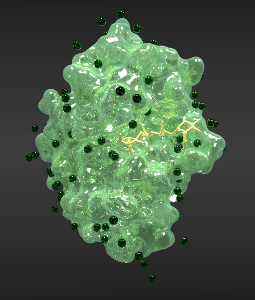
\includegraphics[height=0.5\textheight]{1lmp_2_small.png} 
			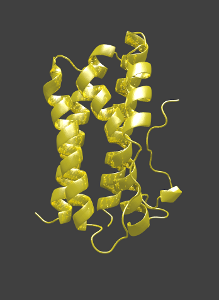
\includegraphics[height=0.5\textheight]{c_gold_small.png} 
			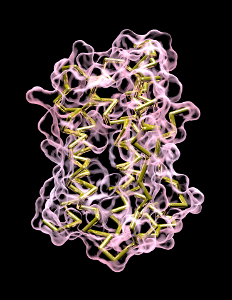
\includegraphics[height=0.5\textheight]{s_s_flame_black2_small.png}
		\end{center}
		\end{frame}

\begin{comment}
	  \begin{frame}{Или рисовать ручкой}
		  \begin{center}
			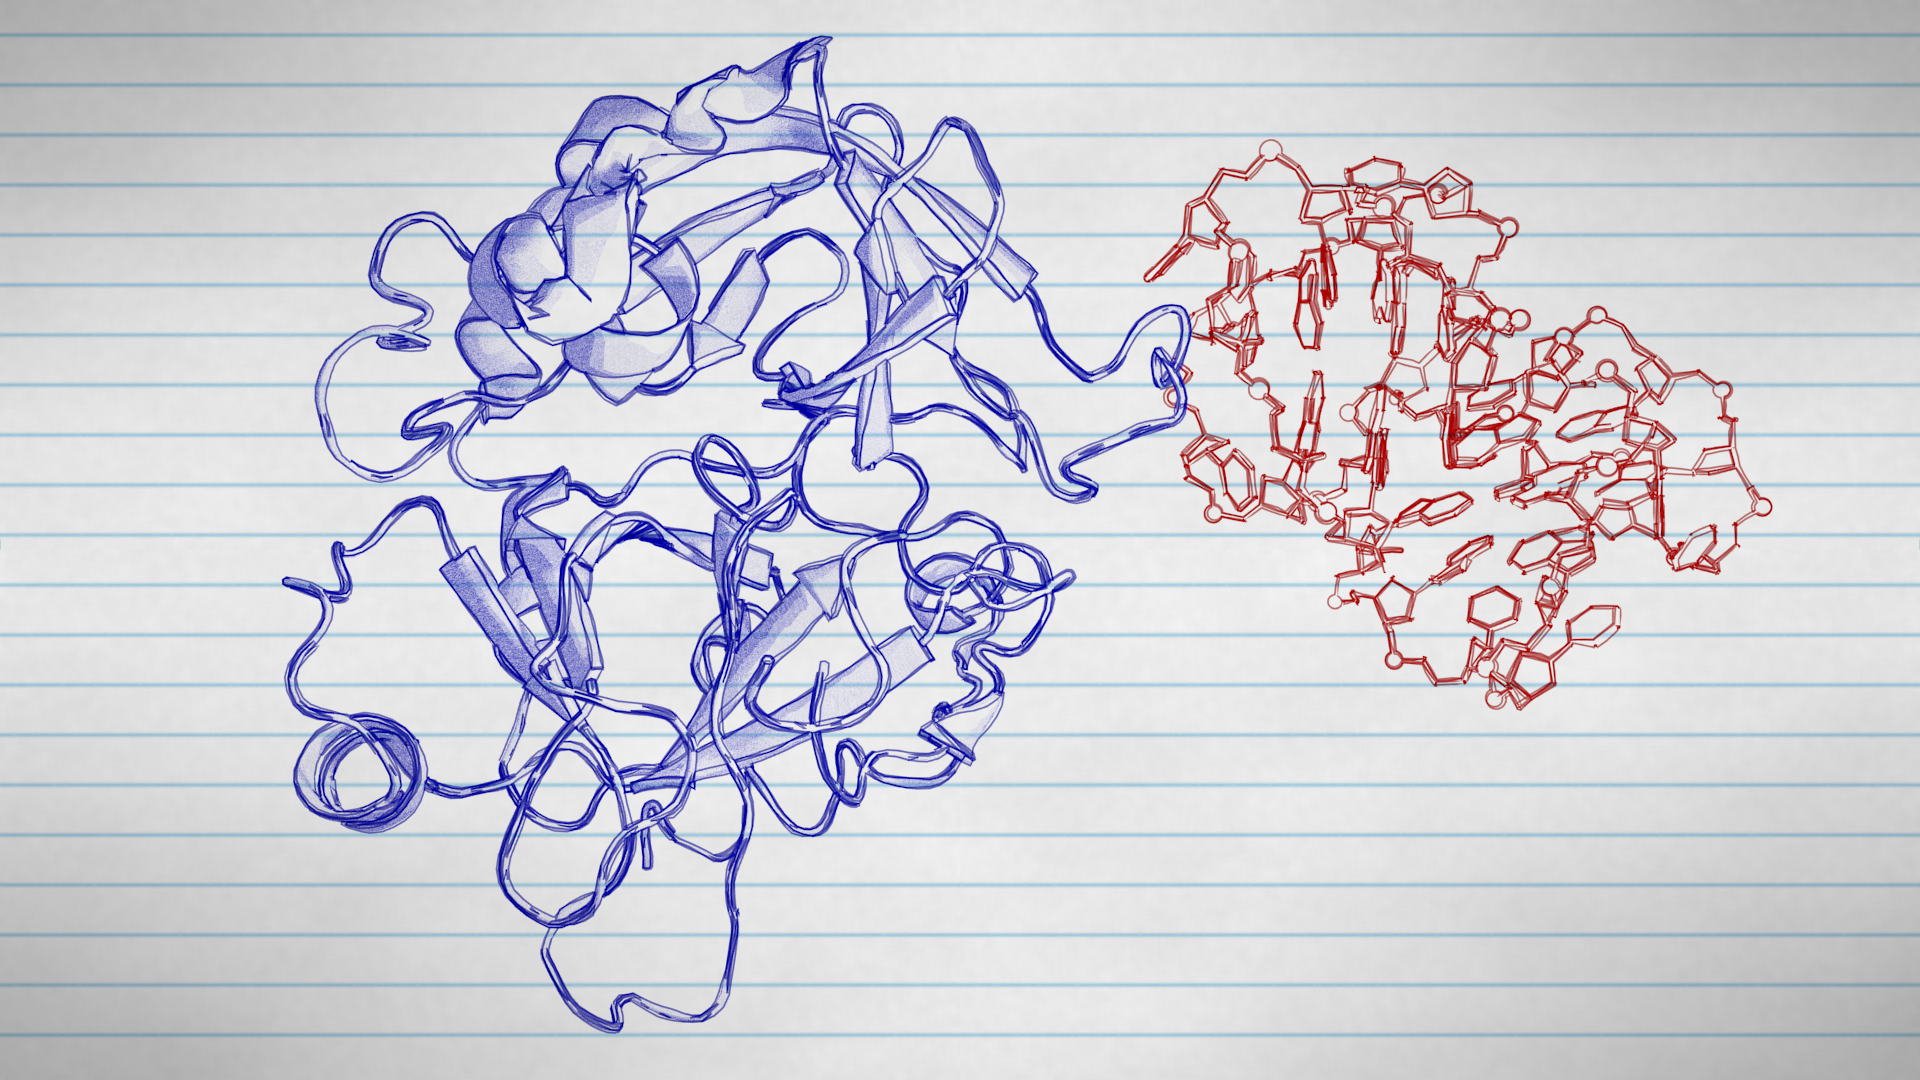
\includegraphics[width=1\textwidth]{sketchy-tamara} 
		\end{center}
		\end{frame}
\end{comment}

	  \begin{frame}[plain]
			\includegraphicsfs{sketchy-tamara} 
	  \end{frame}
\begin{comment}

\begin{frame}[plain]{}
    \begin{textblock*}{\paperwidth}(0\paperwidth,0\paperheight)
    \inlineMovie[loop&autostart]{../../avi/try4_vessel.avi}{surf}{width=1\textwidth}
    \end{textblock*}
\end{frame}
\end{comment}

    \fullFrameMovie[loop&autostart]{../../avi/try4_vessel.mp4}{try4_vessel}{\copyrightText{Анимация структуры в Blender}}
%	  \begin{frame}{Анимация структуры в Blender}
%          \begin{center} 
%    \movie[poster,autostart,width=0.72\linewidth, height=0.4\linewidth,loop]{%
%        \hspace{1cm}\includesvg{media-playback-start}
%           }{../avi/try4_vessel.avi}
%          \end{center}
%		\end{frame}
				  
%%%%%%%%%%%%%%%%%%%%%%%%%%%%%%%%%%%%%%%%
\begin{comment}

\end{comment}


%%===========================
	




\end{document}


